\documentclass[floatfix,aip,rsi,reprint,graphicx]{revtex4-1}
% for checking your page length
%\\documentclass[aip,rsi,preprint,graphicx]{revtex4-1} % for review purposes
\usepackage{amsmath, amssymb}
%\usepackage[numbers]{natbib}
\usepackage{graphicx}
\begin{document} \title{Eliminating centre discrepancies
between simultaneously captured ILIDS and PIV images by means of feature-based 
homography estimation} \author{Sebastian Kosch and Nasser
Ashgriz} \email{\{skosch,ashgriz\}@mie.utoronto.ca} \affiliation{Department of
    Industrial and Mechanical Engineering, University of Toronto}
    \begin{abstract} Interferometric Laser Imaging for Droplet Sizing (ILIDS
        a.k.a. MSI or IPI) requires the objective lens to be defocused so that
        fringe patterns can be imaged. When two cameras are used (e.g. to
        perform simultaneous PIV and ILIDS measurements or to assist in the
        detection of overlapping droplet images) this defocusing introduces a
        distortion that thwarts an accurate calibration of the two cameras
        and makes a successful registration of the two images impossible. To
        overcome the obvious difficulties presented by empirical ad-hoc
        estimates of this ``centre discrepancy'' distortion, we propose that existing keypoint extraction and
        description algorithms can be used on the images directly to find
        homographies. Our approach eliminates the need for camera calibration and leads
        to greatly improved matching between images.
\end{abstract} \maketitle

\section{Introduction} Interferometric Laser Imaging for Droplet Sizing (ILIDS),
also known as IPI (Interferometric Particle Imaging) and MSI (Mie Scattering
Imaging) is an optical droplet sizing method. Its basic principle is based on
the way a laser sheet is scattered by a spherical droplet: from a lateral
perspective, the laser sheet is reflected and refracted into two glare points on
the droplet sphere. When imaged through a lens away from the focal plane, the
glare points---being sources of coherent monochromatic light---cast a circular
fringe pattern, henceforth referred to as a disk. The spatial frequency of the
fringes is (to a very close approximation) linearly related to the particle
size. The phenomenon was first described by \citet{Konig86} and later in greater
detail by \citet{Glover95}.

The ability to image a whole 2D field of droplets all at once, ILIDS' strongest
selling point, is also its curse: when droplets are spaced too closely, their
defocused images overlap and it becomes difficult to determine the fringe counts
corresponding to individual droplets. \citet{Damaschke02} provide a statistical
estimate on the fraction of overlapping disks (overlap coefficient). Arguably
the most popular way to immensely reduce the overlap coefficient is the use of
optical compression techniques, whether by means of a slit aperture\cite{Pan06}
or a cylindrical lens\cite{Kawaguchi02, Maeda02}. However, since some techniques
(e.g. Global Phase-Doppler\cite{Damaschke01} and intensity-analyzing
methods\cite{Querel10}) or situations (e.g. very low signal-to-noise ratios)
rely on the full disk image being available, optical compression/integration is
not always a feasible option. An alternative method of dealing with overlap
attempts to identify the contours of the overlapping disks, either to limit the
fringe frequency analysis to the non-overlapping regions of each disk or to
perform a frequency analysis that takes overlap into account.

\subsection{Calibration and centre discrepancies}

Although a single camera is in theory sufficient to capture an ILIDS image, two
cameras are often used in practice. One important reason is that a focused
image, taken at the same instant as the defocused image, can provide a basis for
the identification of overlapping disks mentioned above. This is the case, for
instance, for the ILIDS system sold by Dantec Inc. Another reason can be the
desire to obtain two different images at once; an example of this is provided by
\citet{Hardalupas10}, who intended to simultaneously capture ILIDS and PIV
images to get size and velocity measurements for the same set of droplets.

To allow both cameras to image the same physical region in the spray, they are
either placed behind a beamsplitter at a right angle to the light sheet, or
placed separately at different angles. The latter approach makes for a more
difficult setup, since Scheimpflug's rule demands that the camera must be tilted
with respect to the objective lens, but it gives the user the freedom to choose
the highest-intensity scattering angle.

In any of the above cases, the use of two cameras requires that their images be
mapped onto one another. This is commonly achieved by means of a camera
calibration procedure, in which a target pattern (e.g. as in FIG.
\ref{fig:plate-calibration}) of known dimensions is
photographed by each camera. A pattern recognition algorithm then determines the
object-to-image mappings for each camera:

\begin{equation}
\left[\begin{array}{c} x'\\ y'\\ z'\\ r' \end{array} \right]
=
\left[ \begin{array}{cccc}
S_x & A_{yx} & A_{zx} & T_x \\
A_{xy} & S_y & A_{zy} & T_y \\
A_{xz} & A_{xy} & S_z & T_z \\
P_x & P_y & P_z & S_0
\end{array} \right]
\left[ \begin{array}{c} x\\ y \\ z \\ 1 \end{array} \right].
\end{equation}
\begin{figure}
    \centering
    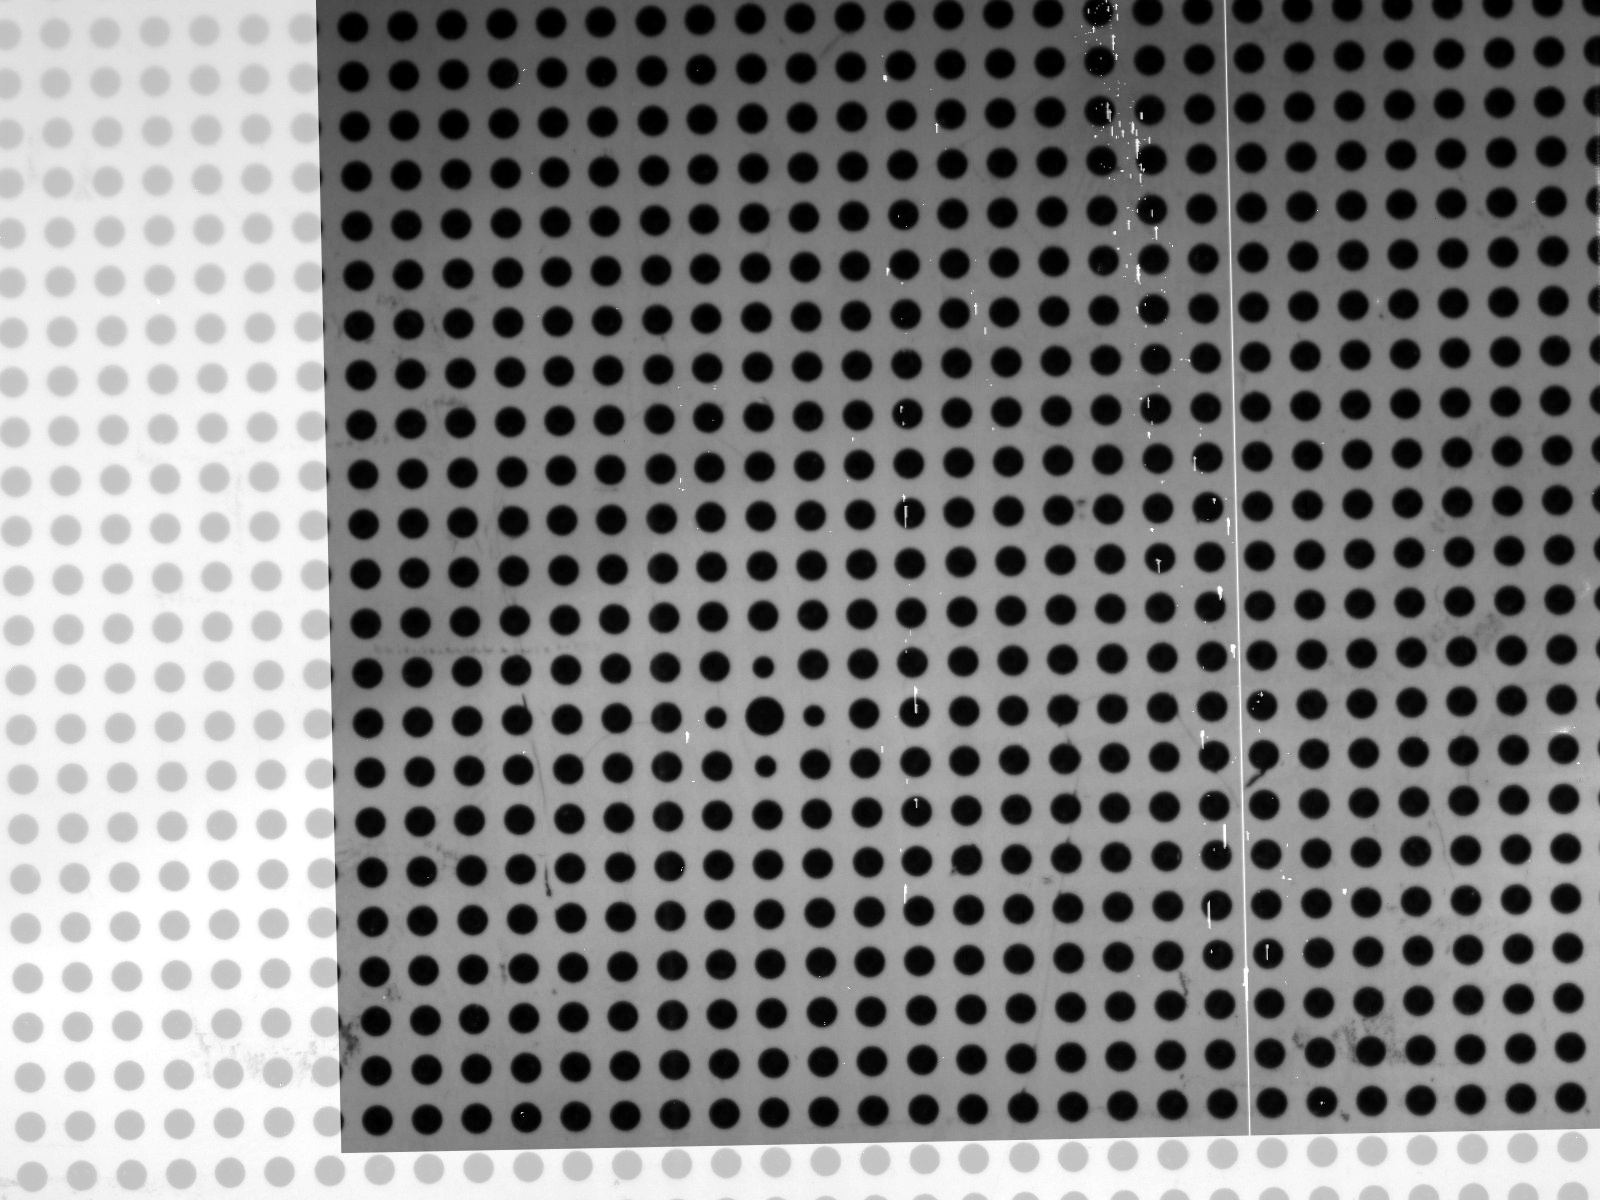
\includegraphics[width=0.46\textwidth]{orb_images/plate-calibration.jpg}
    \caption{Homography $\mathbf{H}$ applied to target pattern image captured by
        the focused camera and superimposed on the image captured by the
        defocused camera (here, both cameras were in focus for the calibration
        only).
    \label{fig:plate-calibration}}
\end{figure}
In practice, $P_{x,y,z} = 0$ and $S_z = S_0 = 1$, such that the mapping is
affine (although we will later show that this need not be the case). The
$z$-components (third row/column) are assumed to be zero, such that a $3 \times 3$ matrix
suffices for the purposes of this discussion:
\begin{equation}
\left[\begin{array}{c} x'\\ y'\\ r' \end{array} \right]
=
\left[ \begin{array}{ccc}
S_x & A_{yx} &  T_x \\
A_{xy} & S_y &  T_y \\
P_x & P_y & S_0
\end{array} \right]
\left[ \begin{array}{c} x\\ y \\ 1 \end{array} \right].
\end{equation}

The calibration algorithm thus finds the camera matrices
$\mathbf{P}_\text{foc}$ and $\mathbf{P}_\text{def}$ mapping the
object coordinates $\mathbf{x}$ onto the two camera images
$\mathbf{x}_\text{foc}'$ and $\mathbf{x}_\text{def}'$ (the respective 
    subscripts shall hence designate the focused and defocused
    cameras):
\begin{align}
    \mathbf{x}_\text{foc}' &= \mathbf{P}_\text{foc} \, \mathbf{x} \\
    \mathbf{x}_\text{def}' &= \mathbf{P}_\text{def} \, \mathbf{x}.
\end{align}

It follows that the quotient of the two matrices, also known as the homography
\begin{equation}
    \mathbf{H} = \mathbf{P}_\text{def} \, \mathbf{P}_\text{foc}^{-1}
\end{equation}
can be used to map the focused image onto the defocused image, as shown in FIG.
\ref{fig:plate-calibration}:
\begin{equation}
    \mathbf{H}\, \mathbf{x}_\text{foc}' = \mathbf{x}_\text{def}'.
    \label{homography-definition}
\end{equation}

Unfortunately, the calibration procedure itself introduces an unwanted
distortion: to capture a viable photo of the target pattern, the defocused
camera must be temporarily brought into focus, as was done in
FIG. \ref{fig:plate-calibration}. This is not mentioned e.g. in the
application manual of Dantec's IPI system, but is a practical necessity.
Bringing a camera out of focus not only introduces a blur, it also scales the
image extents. FIG. \ref{fig:discrepancy}, reproduced from \citet{Hardalupas10},
shows schematically how this effect creates ``centre discrepancies'': since the
extents of the defocused image are either smaller or larger than those of the
focused image, depending on the direction of defocusing, all droplet images are
projected either clsoer to or farther away from the image centre, and the
discrepancy is worst for droplets far away from the image centre. As a result,
the centres of objects in simulatenously captured focused and defocused images
no longer align (FIG. \ref{fig:drop-calibration-off}); the calibration procedure is self-defeating.

\begin{figure}
\centering
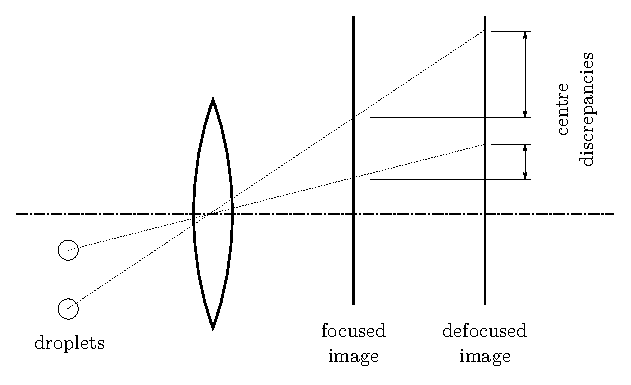
\includegraphics[width=0.45\textwidth]{orb_images/discrepancy.eps}
\caption{Schematic showing the source of centre discrepancies in the case of
parallel image and object planes \label{fig:discrepancy}}
\end{figure}
\begin{figure}
    \centering
    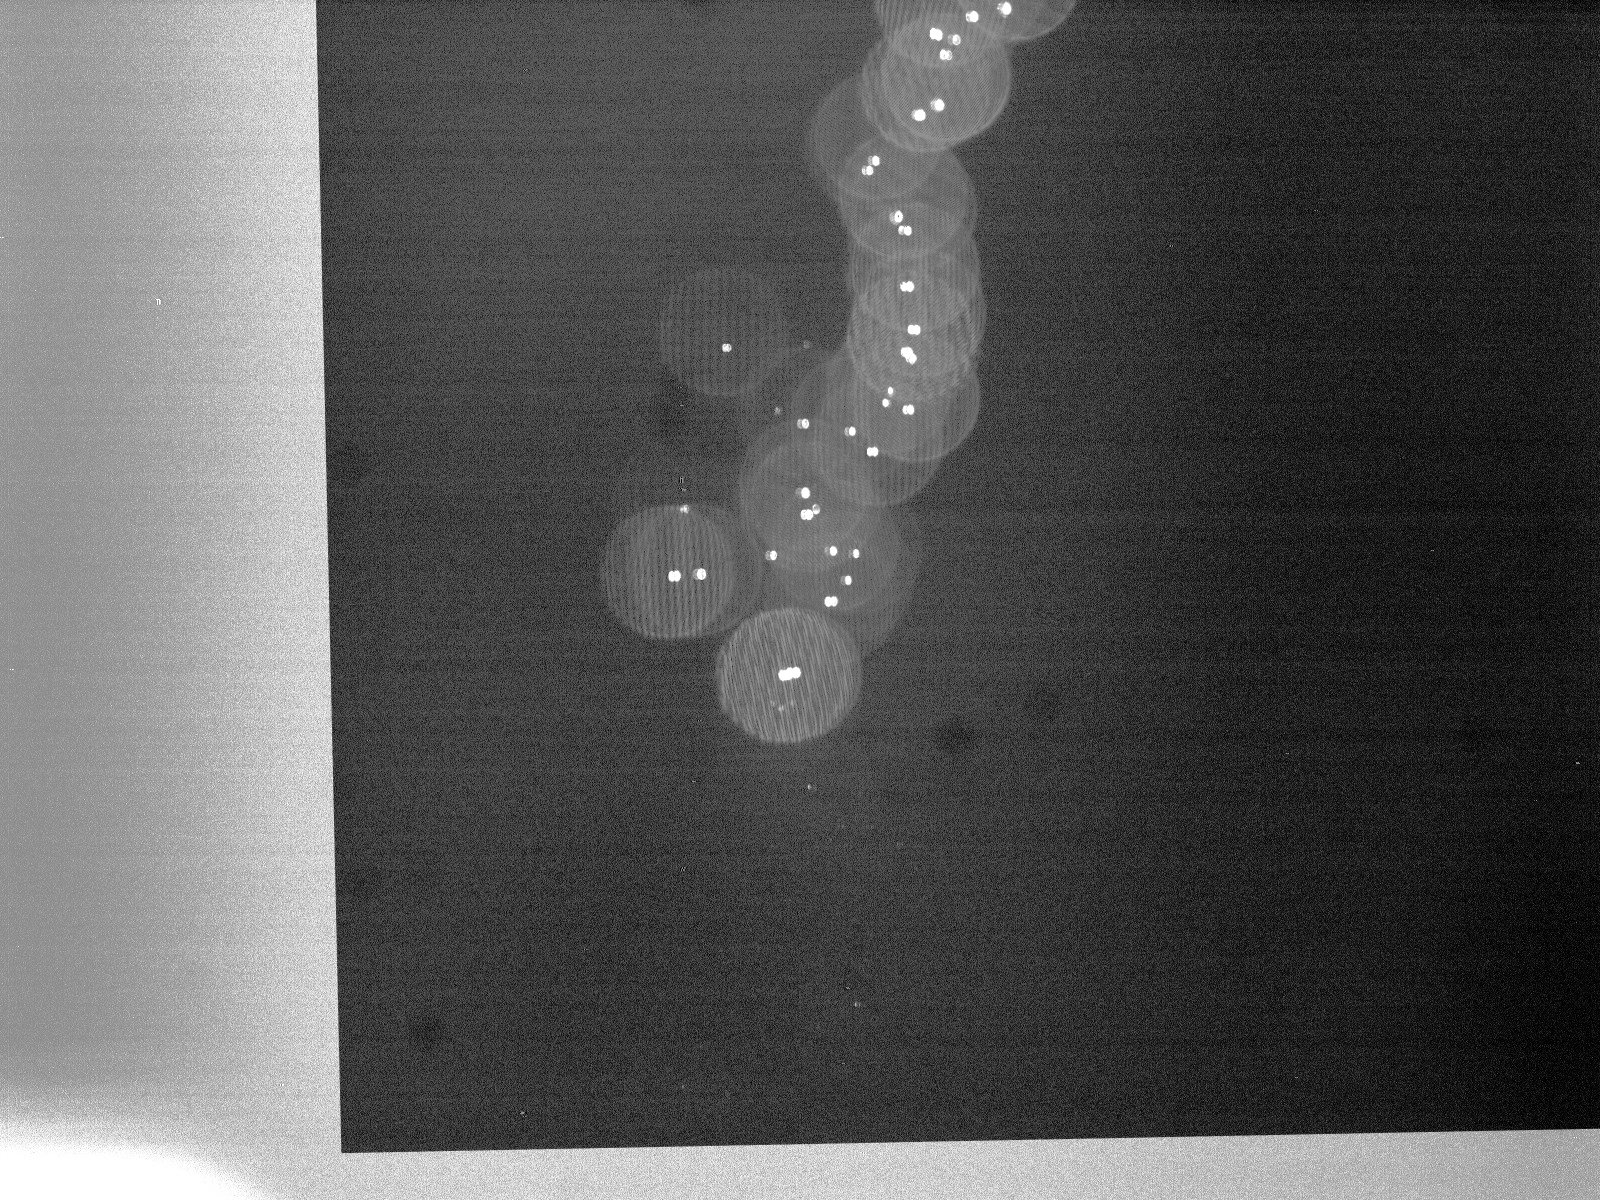
\includegraphics[width=0.45\textwidth]{orb_images/drop-calibration-off.jpg}
    \caption{Focused camera image, after applying homography $\mathbf{H}$
        derived from the calibration images, is superimposed onto
    defocused camera image of droplets. Discrepancies between object centres
grow towards the edge of the image.}
    \label{fig:drop-calibration-off}
\end{figure}
While this error is easy to account for in the ideal case of right angles and
perfect alignments---simply rescaling the image would solve the problem---the
situation becomes more difficult in practice when the target pattern is no longer
parallel to the camera sensor (intentionally or accidentally) or when
cylindrical lenses are used to add optical compression.

\subsection{Context and structure of this paper}
Surprisingly, only \citet{Hardalupas10} have hitherto published a discussion of
this effect, and the only previous mention known to the authors is in
\citet{Kurosawa02}, who dismissed it as a ``positioning error''.

\citet{Hardalupas10} identified the
centres of particles in both PIV (focused) and ILIDS (defocused) images. Then
they empirically estimated the magnitude of the centre discrepancy effect along
the vertical axis, which enabled them to improve the accuracy of their
nearest-neighbour-based centre matching algorithm.

In this article, we show that existing algorithms developed by the computer
vision community in recent years can obviate the need for calibration entirely.
Instead, we can use visual correspondences between the focused and defocused
images to find the mapping between them directly. To that end, we first provide
in Section \ref{sec:review} a brief overview over popular methods in the field of automated (linear)
\emph{registration}, i.e. the art of finding a \emph{homography} (geometric
mapping) between two \emph{epipolar images} (images of the same object, taken
from different positions and angles). Section \ref{sec:results} documents 
our approach in greater detail and shows the result of a successful
recalibration. While our goal was to automatically identify the disk centres in
an uncompressed ILIDS image, the presented algorithms are equally viable candidates for
applications akin to that of \citet{Hardalupas10}; therefore we shall comment on their
setup as well.

\section{Review of image registration techniques \label{sec:review}}
Given two identical images that have been rotated, shifted or even scaled with
respect to one another, the applied transformation can theoretically be found by
means of a brute-force search. This method is not feasible in practice, not only
because of its enormous computational complexity (there are no gradients to
guide the search) but also because of its inability to deal with noise, focal
blur, perspective changes and other nonlinearities introduced by the
photographic process. Conversely, normalized cross-correlation measures between
images, as commonly used in PIV, are unaffected by noise but not invariant to
rotation and scale and therefore not generally practicable. The standard
approach is therefore a three-step process. First, \emph{keypoints}, i.e.
``interesting'' points in the images are found by a keypoint detection algorithm.
Then, a small image patch at every keypoint is extracted and converted into a
\emph{feature vector}, a set of numbers providing a very general description of
the image patch that accounts for scale, rotation, blur, contrast, etc. Finally,
matches between similar feature vectors between the two images are found,
outliers are removed, and the homography is calculated.

An early example of a keypoint detection algorithm is the Harris corner
detector\cite{Harris88}. However, the results of a keypoint detection algorithm
must be as repeatable as possible, i.e. the same set keypoints should be found
in both images regardless of their relative position, rotation, scale, etc. (the
Harris corner detector is sensitive to scale, for instance). The recent decade
has seen a rapidly growing interest in keypoint detectors, beginning with
\textsc{sift}\cite{Lowe04}, \textsc{surf}\cite{Bay08} and \textsc{brisk}\cite{Leutenegger11}, all of which
include keypoint extractors, to \textsc{censure}\cite{Agrawal08}, optimized for speed,
and \textsc{fast}\cite{Rosten05}, which incorporates machine learning methods. Finally,
the recent publication of \textsc{orb}\cite{Rublee11} includes a rotation-aware version
of \textsc{fast} used in this paper. Many more have been developed but are not included
here for brevity's sake.

Keypoint extractors (sometimes called \emph{descriptors}) are often optimized
for and therefore included with keypoint detectors, as in the instances
mentioned above. Some, however, are standalone algorithms such as
\textsc{brief}\cite{Calonder10}.

It is straightforward to find matching keypoint vectors by searching for pairs
with a small arithmetic distance (e.g. using the $L^2$ norm). This nearest-neighbour search
can be done exhaustively in linear time to find the optimal matching, but many
faster, if approximate, search methods exist. We should note \textsc{flann}\cite{Muja09},
a publicly available collection of such implementations which includes a fully
automatic parameter selection heuristic.

Finally, the homography---assuming one exists---can be derived from the set of
matched keypoint coordinate pairs. Since many of the found matches will be
wrong, it is of essence to use a robust estimator, i.e. a type of regression
model designed to ignore outliers. Possibly the oldest of these methods is
\textsc{ransac}\cite{Fischler81}, an iterative procedure in which sets of data points are
chosen at random and discarded if the agreement between a model fit to them and
all other data points falls below a carefully chosen threshold. \textsc{ransac} was used
for this paper, although other robust methods exist. The criterion developed by
\citet{Moisan04} deserves special mention in our context; it does away with
\textsc{ransac}'s hard threshold and instead takes into consideration the probability of
a match to be in consensus with epipolar geometry.

\section{Using affine oriented \textsc{fast}, \textsc{brief} and \textsc{ransac} to estimate the homography
between PIV and ILIDS photographs \label{sec:results}}

Existing PIV/ILIDS systems derive the homography from the result of a camera
calibration procedure which the user is required to perform.
The final value of $\mathbf{H}$ is invisible to the user in our copy of
Dantec's DynamicStudio software, the camera matrices $\mathbf{P}_\text{foc}$ and
$\mathbf{P}_\text{def}$ can be shown and edited. We therefore must find a
corrected homography $\mathbf{\hat{H}}$ that allows us to compute
\begin{equation}
    \mathbf{\hat{P}}_\text{def} = \mathbf{\hat{H}} \, \mathbf{P}_\text{foc}.
    \label{corrected-homography-use}
\end{equation}
We can now replace $\mathbf{P}_\text{def}$ with $\mathbf{\hat{P}}_\text{def}$ in
the software, effectively correcting $\mathbf{H}$ to $\mathbf{\hat{H}}$.

To efficiently extract keypoints, we combined three algorithms:
\textsc{asift}\cite{} to deal with skew transformations; an oriented version of
\textsc{fast}, published as part of \textsc{orb}, to detect keypoints; and
standard \textsc{brief} as a keypoint extractor.

\textsc{asift} is a method originally developed to be used with \textsc{sift}.
It introduces invariance to affine mappings by simulating various
transformations while \textsc{fast} and \textsc{brief} are run repeatedly.
Unsurprisingly, this slows the analysis down, but given the infinitude of
possible angled camera-camera-object configurations, it is wise to maintain a
flexible framework.

We should note that the original \textsc{asift} with
\textsc{sift} works well, but \textsc{sift} is encumbered by patents. To
encourage vendors of imaging systems to adopt the proposed algorithms, we made
it our goal to find a freely available replacement.

Recall that the disks in the defocused image are missing from the focused image,
rendering a registration between them impossible. It is straightforward to
simulate the disks, however. We followed the following protocol on our focused
images:
\begin{enumerate}
    \item Mask the image, blacking out all areas that are known not to contain
        droplets.
    \item Subtract the pixel-wise minimum or mean value taken over all images
        taken by the camera. This step serves to black out defective hot pixels
        on the camera's CCD and other static noise.
    \item Erode the image, using a $3\times 3$ or $5\times 5$ kernel. This will
        close any remaining bright pixels which are likely noise.
    \item Locate the intensity peaks in the remaining image.
    \item Fill a blank image with black, then draw bright circles of diameter
        $D_\text{disk}$ onto it, centred at the respective positions of the
        intensity peaks detected in the focused image. (Note that simply dilating
        the result of the previous step will not lead to circular disks.)
\end{enumerate}
\begin{figure}
    \centering
    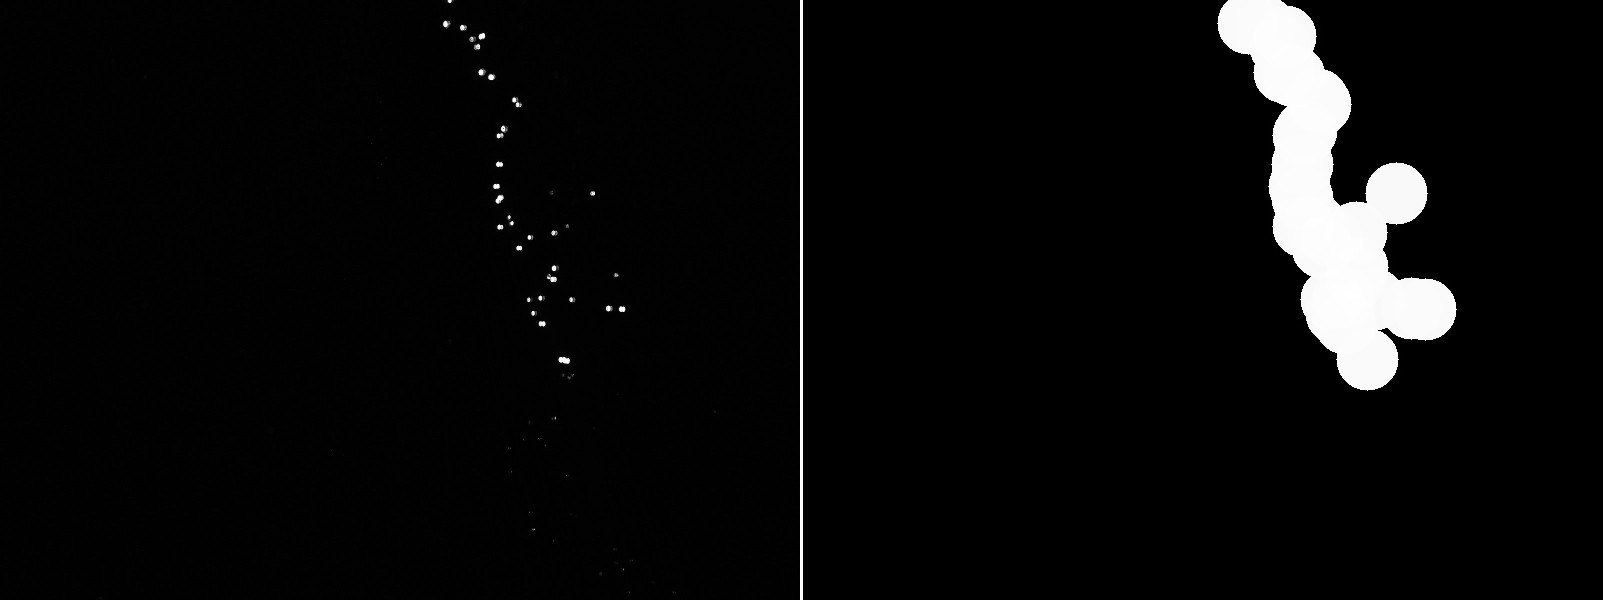
\includegraphics[width=0.5\textwidth]{orb_images/dilation.jpg}
    \caption{Simulating disks based on the focused image. \label{fig:making-disks}}
\end{figure}

The result of performing these operations on our sample image is shown in FIG.
\ref{fig:making-disks}. We determined the disk diameter $D_\text{disk}$
empirically from the defocused images, although it is naturally preferable to
automate this step, e.g. using circular Hough transforms or cross-correlation
with circular masks. There may be simpler ways of achieving the same result,
e.g. by means of Gaussian filters, distance transforms and thresholding
operations. However, we found the protocol described above to be quite robust to
noise and fast enough for our application.

Implementations of \textsc{orb} and \textsc{brief} are freely available through
the OpenCV project, which provides bindings for the C++ and Python languages. We
used these implementations to find and extract matching keypoints between our
sample images, shown in FIG. \ref{fig:matching}.

\begin{figure}
    \centering
    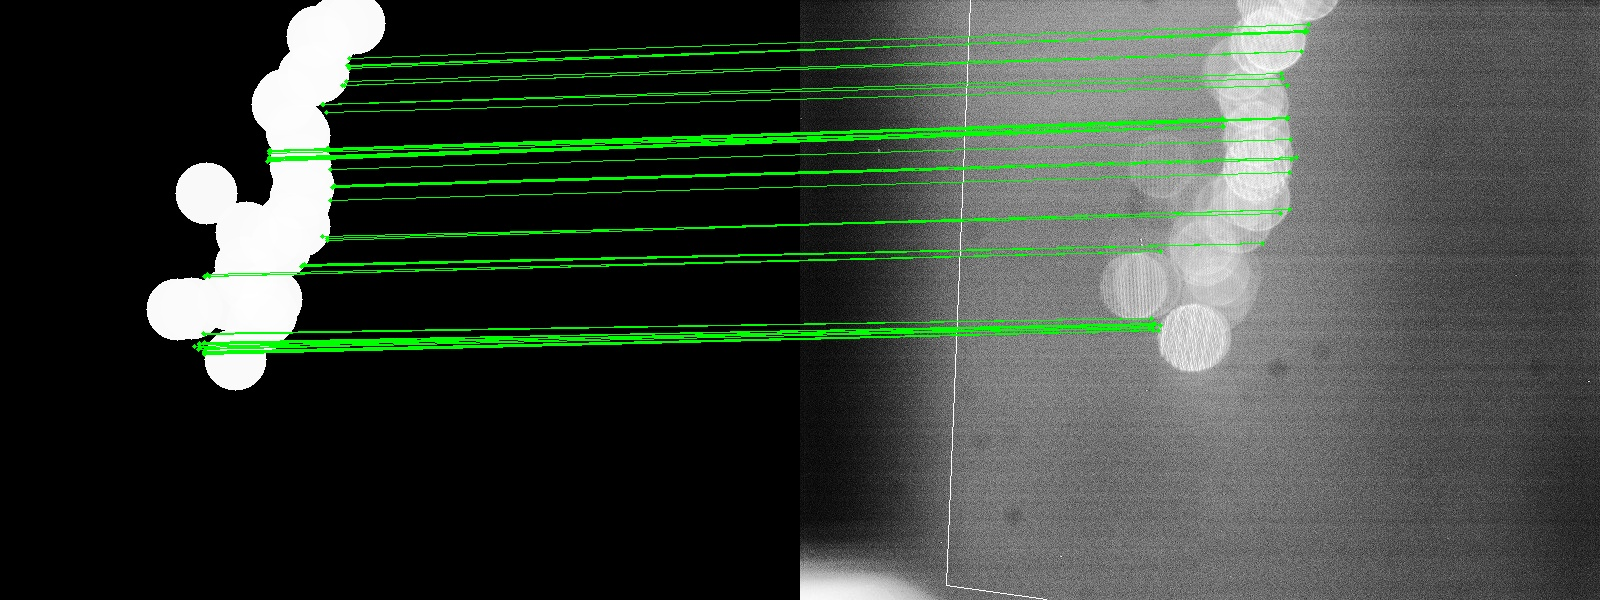
\includegraphics[width=0.5\textwidth]{orb_images/asift-matching.jpg}
    \caption{Visualized inliers in the set of matched keypoints between the
    mirrored simulated disks (see FIG. \ref{fig:making-disks}) and the ILIDS image. \label{fig:matching}}
\end{figure}

The matches shown in FIG. \ref{fig:matching} were found using a most basic
method: brute-force match search, followed by a \textsc{ransac} estimation of the
homography matrix $\mathbf{K}$ using a threshold of 10.

Since the two cameras were positioned behind a beamsplitter in our setup, the
defocused image was flipped horizontally. We therefore first mirrored it
horizontally, using the transformation matrix
\begin{equation*}
    \mathbf{M}_h = \left[ \begin{array}{ccc}
    -1 & 0 & \text{(image width)} \\
            0 & 1 & 0 \\
            0 & 0 & 1
    \end{array} \right].
\end{equation*}

To speed up the image registration process, it can be helpful to first down-scale the
images. To reduce an image to half of its original size, apply
\begin{equation*}
    \mathbf{S}_{0.5} = \left[ \begin{array}{ccc}
    0.5 & 0 & 0 \\
            0 & 0.5 & 0 \\
            0 & 0 & 1
    \end{array} \right].
\end{equation*}

If the registration algorithms mentioned above now find a homography matrix
$\mathbf{K}$, then we can write
\begin{equation}
    \mathbf{K}\, \mathbf{M}_h\, \mathbf{S}_{0.5}\, \mathbf{P}_\text{foc} =
    \mathbf{S}_{0.5} \mathbf{P}_\text{def}
\end{equation}
and to bring this into a form similar to \eqref{homography-definition}, 
\begin{align}
    \mathbf{S}_{0.5}^{-1}\, \mathbf{K}\, \mathbf{M}_h\, \mathbf{S}_{0.5}\,
    \mathbf{P}_\text{foc} &=
     \mathbf{S}_{0.5}^{-1}\, \mathbf{S}_{0.5} \mathbf{P}_\text{def} \\
     &= \mathbf{P}_\text{def}
\end{align}

Finally, it turns out that Dantec's DynamicStudio software violates convention
by placing the coordinate origin at the bottom (not top) left corner of the
image. We must therefore pre- and post-multiply by $\mathbf{M}_v^{\pm 1}$, with
\begin{equation*}
    \mathbf{M}_v = \left[ \begin{array}{ccc}
            1 & 0 & 0 \\
    0 & -1 & \text{(image height)} \\
            0 & 0 & 1
    \end{array} \right],
\end{equation*}
to arrive at our final expression for $\mathbf{\hat{H}}$:
\begin{equation}
    \mathbf{\hat{H}} = \mathbf{M}_v\, \mathbf{S}_{0.5}^{-1}\, \mathbf{K}\,
    \mathbf{M}_h\, \mathbf{S}_{0.5}\, \mathbf{M}_v^{-1}.
\end{equation}
Substitution of $\mathbf{\hat{H}}$ into \eqref{corrected-homography-use} yields
$\mathbf{\hat{P}}_\text{def}$, which can be manually entered into the
DynamicStudio software. FIG. \ref{fig:drop-calibration-corrected} illustrates
how the use of $\mathbf{\hat{H}}$ leads to an improved alignment compared to
FIG. \ref{fig:drop-calibration-off}.

\begin{figure}
    \centering
    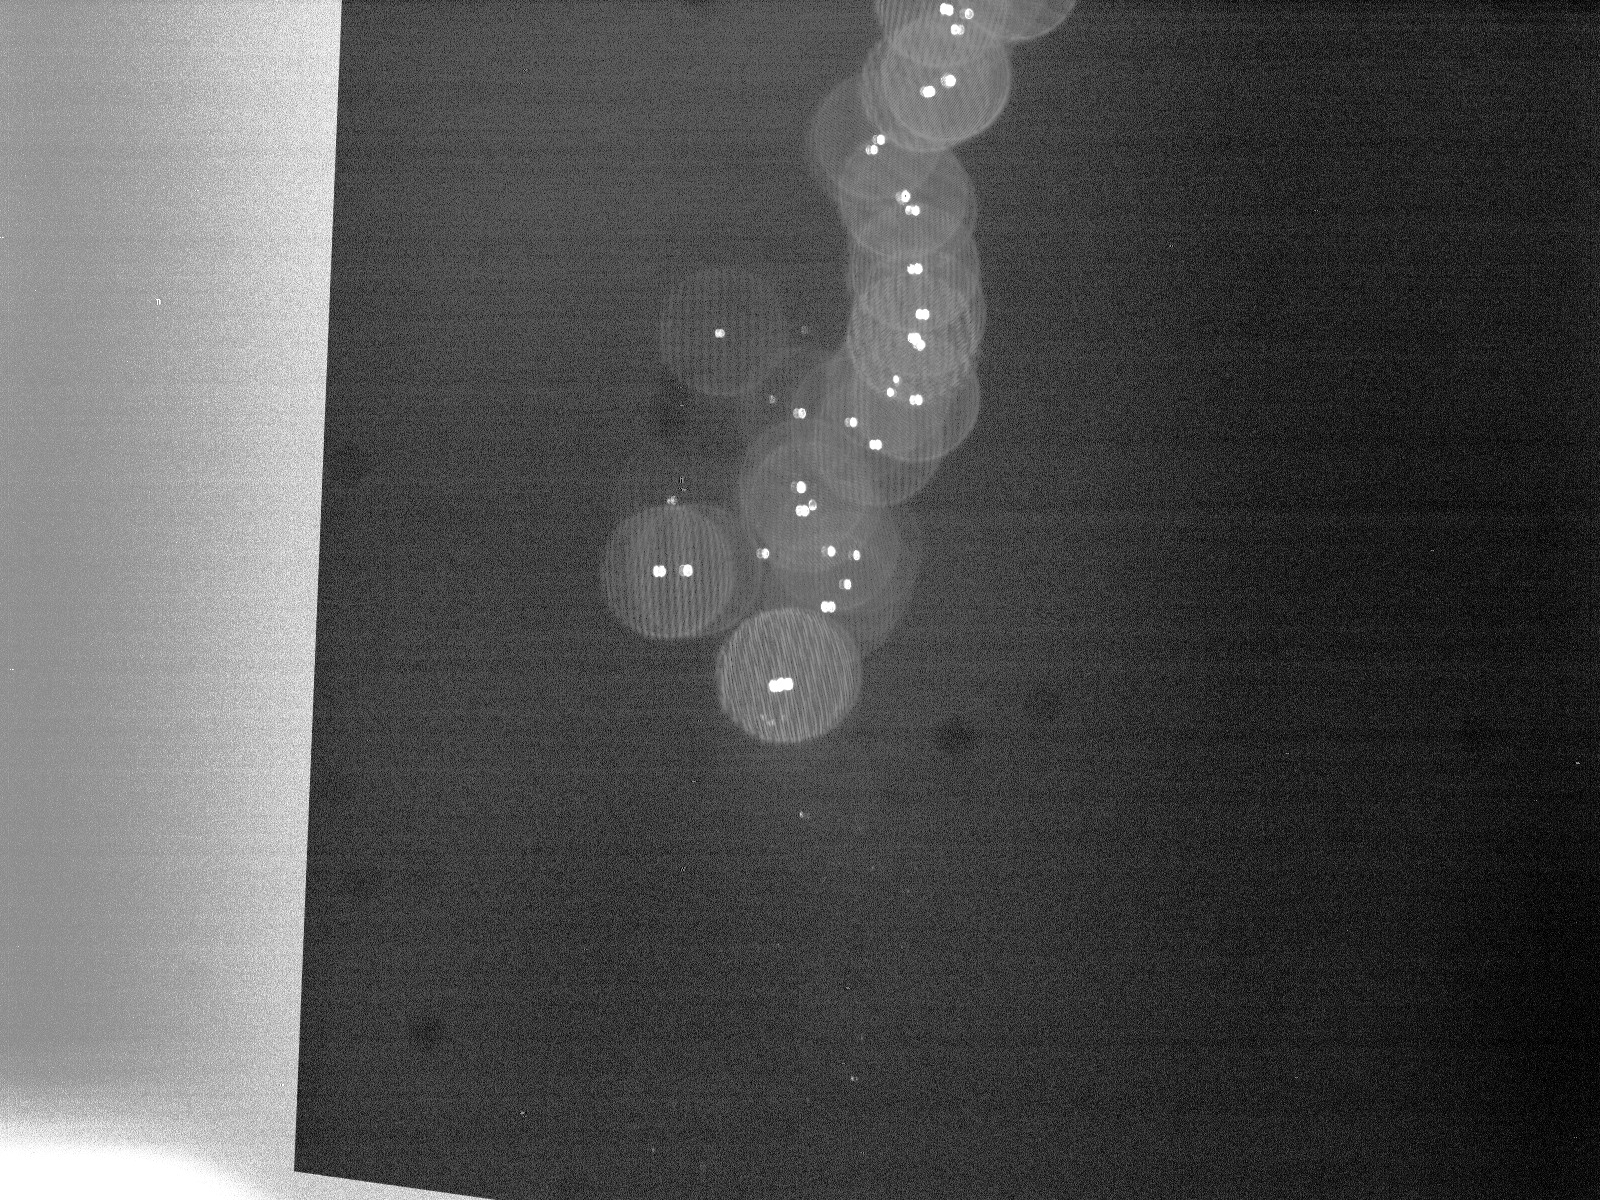
\includegraphics[width=0.45\textwidth]{orb_images/drop-calibration-corrected.jpg}
    \caption{Focused camera image, after applying corrected homography
        $\mathbf{\hat{H}}$ derived from the matched keypoints, is superimposed onto
    defocused camera image of droplets.}
    \label{fig:drop-calibration-corrected}
\end{figure}
\section{Point set registration between PIV and ILIDS centres}
The keypoint matching approach used in the previous section relies on feature
information extracted from the disk images, but those are not available when a
slit aperture is installed to reduce overlap. While slit strip images could be
simulated over the focused image (in a procedure analogous to that illustrated
in FIG.  \ref{fig:making-disks}), the lack of overlap between them will make it
significantly more difficult to find ``interesting'' keypoints. Instead, we can
try to find a direct projection mapping between focused and defocused image
centres.

Indeed, \citet{Hardalupas10} successfully registered their PIV and ILIDS
images that way: using wavelet transforms at various frequencies, they
identified the putative droplet centres on both focused and defocused images.
Then, using a continuous, single-stream monodisperse droplet generator, they
estimated how the magnitude of the centre discrepancies varies over the image.
After applying this empirically estimated distortion, they matched each focused
droplet to the closest defocused droplet (if one can be found within an
subjectively chosen search distance).

Although they reported good success using this method, it requires both an
empirical estimation of the centre discrepancies every time the camera is
defocused \emph{and} a guess at the appropriate search window size. Moreover,
mismatches are likely as the naive closest-neighbour search is not robust to
noise. To eliminate these steps, we suggest that a robust point set
registration algorithm be used.

Since the early 1990s, an impressive body of work on point set registration
methods has accumulated, most of it focusing either on rigid transformations
(i.e. translation and rotation only) or non-rigid transformations (typically
understood to include nonlinear warping). The problem at hand requires an
algorithm able to deal with perspective transforms, which are non-rigid but
linear.

The only paper known to the authors to specifically address this case is by
\citet{Chi11}, who propose an iterative search based on image moments. Since
image moments are an aggregate metric, they do not directly lead to a
droplet-to-droplet correspondence. Still, closest-neighbour matching would
likely produce better results than in the case of an empirically estimated
transformation.

Robust non-rigid methods are also applicable in this case and deserve some
mention. Many of them are a probabilistic relaxations of the Iterative Closest
Point algorithm, which simply searches for the least-squares-optimal rigid
mapping. Several of these approaches were reviewed and generalized by
\citet{Jian10}, who have published a working software implementation. A
variation on their approach, named Coherent Point Drift, is also highly
popular.\cite{Myronenko10}

\section{Conclusion}
Existing image registration algorithms, developed primarily for applications in
robotics and medical imaging, can eliminate the need for camera calibration and 
sidestep the centre discrepancy effect. We have shown how feature-based
registration algorithms can be used to estimate homographies between PIV and
ILIDS disk images, and we have suggested several point set registration methods
to be used in the alignment of images based purely on object centre positions,
e.g. as found in slit-aperture ILIDS images.



\bibliography{orbbibliography}
\end{document}
